\section{Data Conditioning}
\label{sec:conditioning}

\lorena{The training and testing data represent $\sim 200,000$ binary systems comprised
of binary neutron stars (BNS), neutron start-black hole (NSBH), and binary black 
hole (BBH) systems. The data is divided into a training/testing breakdown of
$70\%/30\%$. Regression is applied to four features, namely the initial masses
$m_1, m_2$ and initial spin magnitudes $\chi_1, \chi_2$. Injections are carried
through using LIGO's second observing run (O2) and recovered using the
\texttt{GstLAL}. This low-latency pipeline uses matched-filtering techniques 
for the detection of gravitational-wave signals from compact binaries. 
The template bank of simulated binary neutron stars is generated using the 
TaylorF2 waveform approximant (check all approximants used). The training
datasethas mass ranges $m_1 =  [1.02, 116]$ and $m_2 =  [0.81, 81]$ and spin 
ranges $\chi_{1,2} =  [-0.99, 0.99]$, as shown in 
Fig.~\ref{parameter_space}.}

\begin{figure}
	\centering
	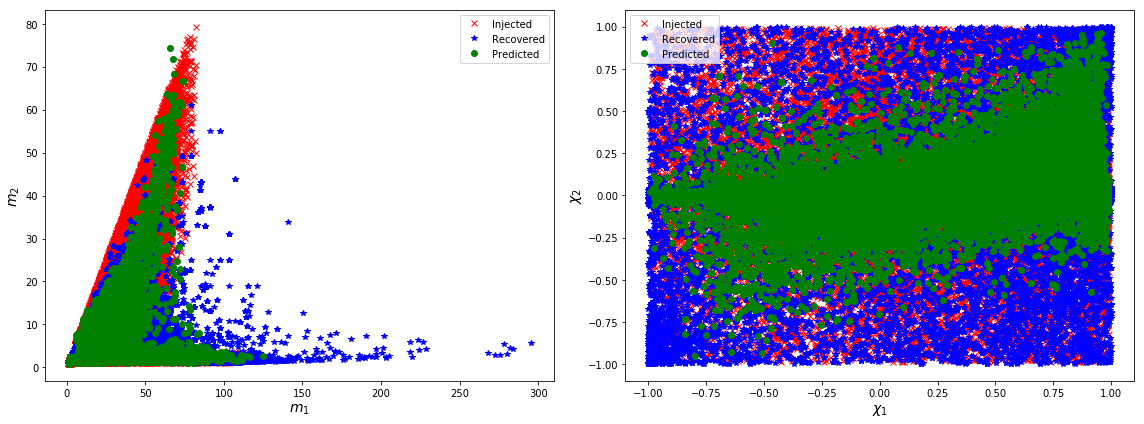
\includegraphics[width=0.45\textwidth]{m1m2_chi1chi2_comparison.png}
    \caption{\lorena{The $m_1$-$m_2$ (left) and $\chi_1$-$\chi_2$ (right) parameter space 
		of injections is shown in red, the recovered
  		values from matched-filtering are in blue, and the predicted values from 
        regression are in green.}}
	\label{parameter_space}
\end{figure}

\lorena{We prepare the data for regression in the following way:}
\begin{enumerate}[label=(\roman*)]
    \item \lorena{Constrain the data to ensure positive values in mass and spin
        predictions. This requires}
	\begin{enumerate}
        \item \lorena{Mapping the data to be in the range from $(0,1)$. This alone does not
			ensure positive values; it is an intermediary step. This is done separately for the
            masses and spins since they span a different range of values.}
        \item \lorena{Mapping the data to be in the range from $(-\infty,+\infty)$.}
	 \end{enumerate}
 \item \lorena{Standardize the data so the data has a zero mean and unit
     variance.}
\end{enumerate}

\lorena{Once the algorithm gives us the predicted data, the reverse process is done, i.e., 
the data is scaled back from standardization, mapped back to $(0,1)$, and
exponentiated.}
